% This file was created by matlab2tikz.
%
%The latest updates can be retrieved from
%  http://www.mathworks.com/matlabcentral/fileexchange/22022-matlab2tikz-matlab2tikz
%where you can also make suggestions and rate matlab2tikz.
%
\definecolor{mycolor1}{rgb}{0.00000,0.44700,0.74100}%
\definecolor{mycolor2}{rgb}{0.85000,0.32500,0.09800}%
\definecolor{mycolor3}{rgb}{0.92900,0.69400,0.12500}%
%
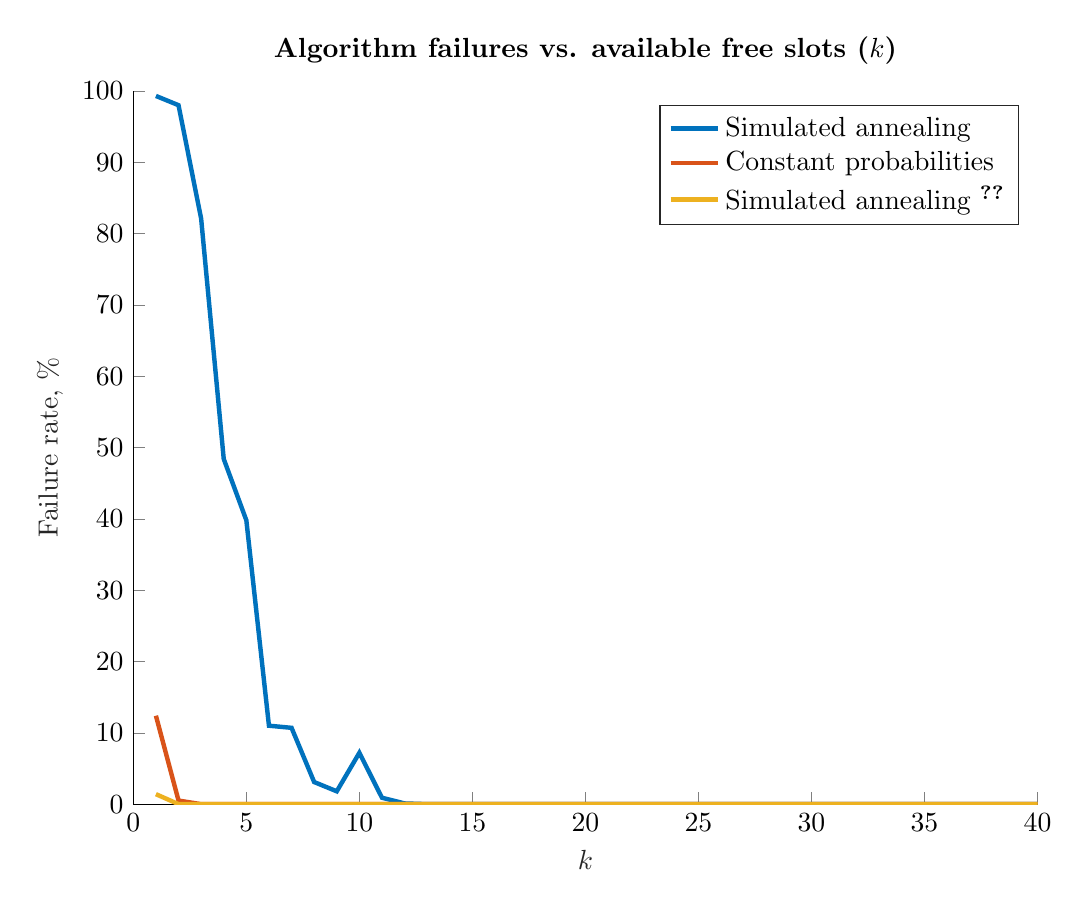
\begin{tikzpicture}

\begin{axis}[%
width=4.521in,
height=3.566in,
at={(0.758in,0.481in)},
scale only axis,
xmin=0,
xmax=40,
xlabel style={font=\color{white!15!black}},
xlabel={$k$},
ymin=0,
ymax=100,
ylabel style={font=\color{white!15!black}},
ylabel={Failure rate, \%},
axis background/.style={fill=white},
title style={font=\bfseries},
title={Algorithm failures vs. available free slots ($k$)},
axis x line*=bottom,
axis y line*=left,
every axis plot/.append style={ultra thick},
legend style={legend cell align=left, align=left, draw=white!15!black}
]
\addplot [color=mycolor1]
  table[row sep=crcr]{%
1	99.3\\
2	98\\
3	82.1\\
4	48.4\\
5	39.8\\
6	11\\
7	10.7\\
8	3.09999999999999\\
9	1.8\\
10	7.2\\
11	0.900000000000006\\
12	0.0999999999999943\\
13	0\\
40	0\\
};
\addlegendentry{Simulated annealing}

\addplot [color=mycolor2]
  table[row sep=crcr]{%
1	12.4\\
2	0.5\\
3	0\\
40	0\\
};
\addlegendentry{Constant probabilities}

\addplot [color=mycolor3]
  table[row sep=crcr]{%
1	1.4\\
2	0\\
40	0\\
};
\addlegendentry{Simulated annealing \textsuperscript{\ref{footnote.1}}}

\end{axis}
\end{tikzpicture}%